\section{Búsqueda de contrastes}

% Definir que es un contraste, que tiene un uso significativo en una region más que en otra. LAs alternativas que propusimos, z test binomial.
Una palabra tiene un contraste cuando tiene un uso con diferencias significativas en
distintas regiones. En este trabajo nos propusimos crear un listado con palabras con contrastes que tengan
importancia a nivel lingüístico. En este sentido, los nombres de personas, lugares u organizaciones no 
fueron considerados de interés a pesar de tener contrastes en su uso.
Este listado fue ordenado por una métrica que capte en un único valor el nivel contrastivo. De esta manera, 
se seleccionó un subconjunto de palabras, de acuerdo a la métrica, el cual fue analizado manualmente por los investigadores de la Academia Argentina de Letras (AAL).

El primer acercamiento para ver el contraste de las palabras surgió de comparar las frecuencias de las palabras 
en cada par de provincias de la Argentina. Para esto calculamos, por cada palabra $w$, la frecuencia de ocurrencias sobre cada una de las dos provincias $p_1$ y $p_2$. A la mayor frecuencia de ambas, la llamamos frecuencia máxima y a la menor, la frecuencia mínima. Luego el cociente entre la \textit{frecuencia máxima} y la \textit{frecuencia mínima} tiene como resultado lo que llamamos \textit{maxDif}. En caso de que en una de las dos provincias no se hayan recolectado tuits con esa palabra, se toma como frecuencia mínima a la frecuencia mínima distinta de 0 de todas las palabras generadas en esa provincia. Así se evitó la división por cero. Esta métrica se resume en la ecuación \ref{eq:maxDif}, siendo $frec(w,p)$ igual a la frecuencia de la palabra $w$ en la provincia $p$.


\begin{equation}
  \label{eq:maxDif} 
  maxDif(w,p_1,p_2) = \frac{f_{max}(w,p_1,p_2)}{f_{min}(w,p_1,p_2)}
\end{equation}
donde 
\begin{equation}
f_{max}(w,p_1,p_2) = \max (frec(w,p_1),frec(w,p_2))
\end{equation}

\begin{equation}
 f_{min}(w,p_1,p_2) = \left\{ \begin{array}{lll}
             \min \left(frec\left(w,p_1\right),frec\left(w,p_2\right)\right), & \text{si } frec(w,p_1) * frec(w,p_2) > 0  & \\
             \\
             \min\limits_{w \in W(P_{min})} frec\left(w,P_{min}\right) , &  \text{si no.} &  \\
             \end{array}
   \right.
\end{equation}
   donde $P_{min}$ es la provincia que tiene la menor frecuencia de ambas y $W(P_{min})$ son las palabras mencionadas en esa provincia.



De esa manera se ordenó el listado de cada par de provincias teniendo en cuenta la división de frecuencias. 
Sin embargo, este método imposibilitaba el trabajo manual para los investigadores de la AAL, que debían mirar estos listados y hacer un análisis más exhaustivo sobre las palabras con mayor diferencia de frecuencias, debido a que había $\binom{23}{2} = 253$
listados (o equivalentemente 253 columnas en un mismo listado) a analizar. Además la métrica solo permitía saber si había un contraste entre dos provincias, pero no se podía tener en cuenta la frecuencia de la palabra en el resto de las provincias. 
% Mencionar que la idea era realizar un z test para obtener las palabras más significativas.
En consecuencia las palabras se encontraban repetidas en los distintos listados y con diferentes valores de \textit{maxDif}, lo cual hacía muy difícil poder identificar en qué regiones había una diferencia significativa de frecuencias.
Debido a esto decidimos realizar un nuevo enfoque para encontrar las palabras con alta contrastividad en las distintas regiones, de manera que una métrica pudiera reflejar el nivel de contrastividad de la palabra en un único valor. 

En primer lugar intentamos modificar la métrica \textit{maxDif} de la siguiente manera. 
Sea $f_{max}^\prime(w)$ la frecuencia máxima de la palabra $w$ entre las frecuencias de todas las provincias y sea $f_{min}^\prime(w)$ la frecuencia mínima distinta de $0$ sobre todas las provincias, luego la métrica generalizada \textit{$maxDif_g(w)$} se puede definir como en la ecuación \ref{eq:maxDifg}.

\begin{equation}
 maxDif_g(w) = \frac{f_{max}^\prime(w)}{f_{min}^\prime(w)}
 \label{eq:maxDifg}  
\end{equation} 

Si bien esta métrica logra resumir en un único valor la diferencia de frecuencias, sigue sin considerar la dispersión de las frecuencias en todas las provincias.
Por este motivo, nos enfocamos en analizar el contraste de frecuencias de palabras sobre las provincias a través de una métrica superadora.

\subsection{Métricas para medir el contraste en la frecuencia de las palabras}
Dado que se quieren encontrar las palabras con contrastes significativos en distintas 
regiones se propone generar una métrica basada en la cantidad de información 
para poder realizar esta tarea.

Una medida que se puede usar para comparar las frecuencias de las palabras en las diferentes regiones del país es la entropía definida por Shannon (ver el Apéndice \ref{sub:entropiaShannon}), debido a que nos brinda un valor que indica qué tan uniforme es la distribución de las frecuencias de cada palabra. La entropía es máxima cuando los eventos son equiprobables y mínima en el caso que la probabilidad de un evento es 1.

Sin embargo, la entropía como única medida tiene sus desventajas. En particular, una palabra con una sola ocurrencia en una provincia y ninguna en las demás, tiene la entropía mínima, lo cual la pondría en igualdad de condiciones con una palabra con 1000 ocurrencias en una única provincia, algo no deseable.

A pesar de que nos interesan las palabras con un contraste significativo entre regiones, dentro de ellas elegiremos las que tienen mayor cantidad de ocurrencias. Es por esto que elaboramos otra métrica que tenga en cuenta la entropía, entre otras variables.


\subsection{Valor de información}
La métrica que utilizamos para ordenar los listados de palabras y detectar cuáles son
las que tienen altos contrastes en su uso en distintas regiones fue inspirada por el
trabajo de Zanette y Montemurro \cite{montemurro2010towards}.
Ellos, a diferencia de Shannon, estudiaron una relación entre una medida de la información y su función semántica en el lenguaje.
A continuación detallamos el procedimiento para calcular lo que los autores llamaron
el \textit{valor de la información}:

% Dado un texto dividido en $P$ partes iguales llamadas \textit{ventanas}, se calcula la entropía  $H(\omega)$ sobre el vector de cantidad de ocurrencias en cada una de las $P$ ventanas.
% Por otro lado, se define $\widehat{H}(\omega)$ como la entropía sobre un reordenamiento aleatorio de todas las palabras del texto, promediada sobre todas las posibles permutaciones de las palabras. Formalmente, sea $(X_{1},\dots,X_{23})$ un vector aleatorio con $X_{i}$ igual a la cantidad de ocurrencias de la palabra $\omega$ en la ventana $i$ en un corpus con una determinada distribución de frecuencias para cada palabra y sea $X^\prime = H(X_1,\dots,X_{23})$. Luego se define $\widehat{H}(\omega) = \mathbb{E}(X^\prime)$, es decir la esperanza de $X^\prime$. Por lo tanto, $\widehat{H}(\omega)$ es el resultado de calcular la media de $H(\omega)$ entre todas las posibles permutaciones del texto.

%%%%%%%%%%%%%%%%%%%% Explicación H y \widehat{H} %%%%%%%%%%%%%%%%%%%%
Dado un texto dividido en $V$ partes iguales llamadas \textit{ventanas}, se calcula la entropía  $H(w)$ sobre el vector de probabilidad de ocurrencia de $w$ en cada una de las $V$ ventanas.  Es decir, $H(w) = -\sum\limits_{i=1}^{V} \frac{w_i}{N_w} * \log(\frac{w_i}{N_w})$ con $N_w$ igual a la cantidad total de ocurrencias de la palabra $w$ en toda el corpus y $w_i$ la cantidad que se obtuvo en la ventana $i$ en el conjunto de datos recolectado. Notar que $\frac{w_i}{N_w}$ es una estimación de la probabilidad de ocurrencia de la palabra $w$ en la ventana $i$. Por otro lado, $\widehat{H}(w)$ es un promedio de $H(w)$ sobre todas las posibles permutaciones de las palabras del texto. Formalmente, sea $\widetilde{W} = (w_{1},\dots,w_{V})$ un vector aleatorio con $w_{i}$ igual a la cantidad de ocurrencias de la palabra $w$ en la ventana $i$. Luego $\widehat{H}(w) = \mathbb{E}[H(\widetilde{W})]$.
Si bien Zanette y Montemurro dividen un texto en $V$ ventanas que pueden variar dependiendo del tamaño de la ventana fijado, en este trabajo se tomo como ventana todos los textos provenientes de una provincia.


Es de esperar que en la mayoría de los casos 
la entropía sobre todas las permutaciones del texto sea mayor que la medida en el cálculo original. Esto 
se debe a que en una gran cantidad de las permutaciones las palabras se distribuyen de forma más uniforme 
en las distintas partes.

Zanette y Montemurro definieron al \textit{valor de la información de una palabra} como
 \begin{equation}
  \Delta I(w) = p(w) \,  (\widehat{H}(w) - H(w))  =  p(w) \, \Delta{H(w)}
 \end{equation}
siendo $p(w)$ la frecuencia total de la palabra en el texto.
De esta manera se les da más importancia a las palabras que son más frecuentes y a las palabras que tienen una baja entropía, ya que en estas el término de la diferencia es más grande.

Los autores analizaron el valor de la información de las palabras sobre tres textos, \textit{Análisis de la mente} de Bertrand Russell, 
\textit{Moby Dick} de Herman Melville y \textit{El origen de las especies} de Charles Darwin. 
En los tres libros las palabras con mayor valor de la información están 
altamente relacionadas con los temas principales. 

% Si bien esta métrica tiene en cuenta la frecuencia de las palabras además de la 
% entropía, el texto en Twitter resulta difícil de dividir en partes iguales. 
% Esto es porque la división está pensada para dividir el texto en secciones que 
% posiblemente hablen de distintos temas y nuestros textos son tuits que por lo general no superan las 10 palabras.

Zanette y Montemurro utilizaron el \textit{valor de la información de una palabra} de manera tal que sumando el valor para todas las palabras $W = \{w_1,\dots,w_K\}$ se obtiene el \textit{valor de información de la distribución de las palabras} $\Delta I(s)$ definido en la ecuación \ref{eq:delta_s}, siendo  $s = N/V$, N la cantidad de palabras en el texto, $V$ la cantidad de ventanas en la que se dividió y $p(w)$ la frecuencia total de la palabra en el texto.

\begin{equation}
  \Delta I(s) = \sum\limits_{w \in W } p(w) (\widehat{H}(w) - H(w)) = \sum\limits_{w \in W } p(w) \Delta H(w) 
  \label{eq:delta_s}
\end{equation}

Zanette y Montemurro definieron esta medida para \textcquote[p. 136]{montemurro2010towards}{cuantificar la relación entre las heterogeneidades de la distribución de palabras debido a su función lingüística y la partición de texto}. De esta manera, para cada texto buscaban cual era el valor de $s$ tal que la información $\Delta I(s)$ sea máxima.
% Este valor lo definieron con el objetivo de maximizar el tamaño óptimo de las $P$ ventanas y así cuantificar la información, sobre partes específicas del texto, es contenida en la distribución de las palabras con respecto al texto aleatorio.


Si bien el \textit{valor de la información de una palabra} definida por Zanette y Montemurro es muy bueno a la hora de calcular el tamaño óptimo de ventana que maximice el valor de la información de un texto $\Delta I(s)$, también refleja un valor que no es conveniente al hacer la comparación entre dos palabras cuando una de ellas es demasiado frecuente (como la palabra \textit{que}). Esto sucede ya que las palabras, al tener valores de frecuencias muy distintos (ver más detalle de esto en la sección \ref{sub: frecuenciaPalabras}), generan un valor de $\Delta I$ muy alto en las palabras más frecuentes en comparación con el resto. Este fenómeno se pone en evidencia en la Tabla \ref{tab:zanette} donde se observa que palabras como \textit{que} y \textit{me} tienen los valores máximos de la métrica $\Delta I$.



\begin{table}[ht]
\centering

\begin{tabular}{ c c }
\toprule
Palabra  & $\Delta I$                      \\
\midrule
que      & 109932.23                         \\
me       & 101754.11                        \\
rioja    & 59244.90                          \\
a        & 54872.75                          \\
re       & 52207.93                          \\
no       & 51470.18                          \\
la       & 47693.43                          \\
de       & 44035.71                          \\
ushuaia  & 42972.62                          \\
jujuy    & 39087.57                          \\
salta    & 33310.16                          \\
el       & 32628.74                          \\
q        & 32596.95                          \\
y        & 29905.83                          \\
comodoro & 25902.79                         \\
\bottomrule
\end{tabular}
\caption{\ref{tab:zanette} Las 15 palabras con mayor valor de $I_w$ }
\label{tab:zanette}
\end{table}

Es por esto que, entre otras cosas, usamos al logaritmo sobre las cantidades de ocurrencias para generar una mejor dispersión de los datos. Así agrupamos a las palabras con un valor de $\Delta H(w)$ parecido y le restamos relevancia a las palabras sumamente frecuentes. Otra dificultad que surge de la métrica propuesta por Zanette y Montemurro es la imposibilidad de realizar la media de todas las posibles permutaciones del texto por la limitación computacional ya que 
tenemos una cantidad muy grande de datos. Es por eso que diseñamos una métrica similar basada en una aproximación de la esperanza de la entropía de una palabra.
% Podemos pensar para cada palabra del corpus, una variable aleatoria que mida el total de la cantidad de ocurrencias en  las palabras del texto como una variable aleatoria $W$, donde cada palabra $w$ tiene una probabilidad de aparición en una provincia dada de la Argentina. Esta probabilidad la aproximamos con la frecuencia en la que aparece, es decir la cantidad de ocurrencias de la palabra dividida por la cantidad de palabras totales.
% Por otro lado sea $P$ una variable aleatoria que cuenta la cantidad de personas que 
% utilizan la palabra $p$ en cada provincia.

% Podemos pensar para cada palabra $w$ que hay una variable aleatoria que mide la cantidad de apariciones de $w$ en toda la Argentina. Del mismo modo, podemos definir una variable aleatoria que cuenta la cantidad de personas que utilizan la palabra $w$ en todo el país.

Sea $\# w$ la cantidad de ocurrencias de la palabra $w$ en toda la Argentina y $W$ todas las palabras posibles en todo el país, definimos
% defino $m_w = \min \limits_{w \in W} \# w$ y del mismo modo defino $M_w = \max \limits_{w \in W} \# w$. Luego, aplico la normalización lineal de $\log(\# \omega)$,


\noindent\begin{minipage}{.5\linewidth}
\begin{equation}
  m = \min \limits_{w \in W} \# w
\end{equation}
\end{minipage}%
\begin{minipage}{.5\linewidth}
\begin{equation}
  M = \max \limits_{w \in W} \# w
\end{equation}
\end{minipage}\\

Luego, realizamos una normalización lineal de $\log(\# \omega)$ 
\begin{equation}
  norm_w(w) = \frac{\log \left(\# w\right) - \log \left(m\right)}{\log \left(M\right) -\log \left(m\right)}
\end{equation}



% Luego, sea $cant_w(w)$ igual al logaritmo sobre la cantidad de ocurrencias de la palabra $w$ en toda la Argentina, es decir $cant_w(w) = \log_2(cantidadOcurrencias(w))$ y sean las constantes $MIN_w$ y $MAX_w$ definidas de la siguiente manera:

% \begin{equation}
% MIN_w = \min\limits_{p \in Palabras} cant_w(w)
% \end{equation}

% \begin{equation}
%   MAX_w = \max\limits_{p \in Palabras} cant_w(w)
% \end{equation}

% Realizamos una normalización lineal de la función $cant_w$, 

% \begin{equation}
% norm_{w}(p) = \frac{cant_w(p)- MIN_w }{MAX_w - MIN_w}
% \label{eq:norm1}
% \end{equation}

Así $norm_w$ tiene su imagen en el rango $[0,1]$, tomando el valor $1$ sobre la palabra que tiene la cantidad de ocurrencias máxima y el valor $0$ cuando se aplica a la palabra con menor cantidad de ocurrencias. Vale la pena aclarar que tomamos $40$ como umbral mínimo de la cantidad de ocurrencias de las palabras para ser estudiadas, por lo tanto $m_w = 40 $.
A partir de la función $norm_w$ definimos el \textit{valor contrastivo sobre las palabras} $I_w$ como:

% \begin{equation}
% I_w(\omega) = \underbrace{norm_{w}(\omega)}_\text{``frecuencia"} \cdot (\underbrace{\widehat{H}_{w}(\omega)}_\text{uso al azar} - \underbrace{H_{w}(\omega)}_\text{uso espec\'ifico}) \\
% % \label{eq:iw}
% \end{equation}

\begin{equation}
I_w(w) = norm_{w}(w) \cdot (\widehat{H}_{w}(w) - H_{w}(w)) \\
\label{eq:iw}
\end{equation}


\noindent siendo $H_w(w)$ la función de entropía calculada sobre las cantidades de ocurrencias de la palabra $w$ sobre las 23 provincias argentinas. Como $\widehat{H_w}(w)$ es un promedio de $H(w)$ sobre todas las posibles permutaciones del texto, al ser este de gran tamaño resulta muy difícil de computar. Es por esto que simulamos la cantidad de ocurrencias de la palabra $w$ en todas las provincias con una distribución multinomial $M(N_w,\frac{1}{23}\ldots,\frac{1}{23})$ y realizamos un promedio de la entropía sobre las ocurrencias simuladas para aproximar $\widehat{H_w(w)}$. Elegimos esta distribución con igual probabilidad de ocurrencia en todas las provincias, para simular el hecho de que todas las palabras ocurren de manera uniforme a lo largo del país.
%De forma similar $\widehat{H_w}(w)$ es la función de entropía sobre las cantidades de ocurrencias simuladas en todas las provincias a partir de una distribución multinomial. Elegimos esta distribución ya que con esta se distribuye la suma de los valores de la variable aleatoria, en nuestro caso la cantidad de ocurrencias de la palabra $\omega$, de forma uniforme.%TODO: explicar más en detalle

\subsection{Robusteciendo la métrica desarrollada}

Ahora bien, una determinada provincia o región puede tener muchas ocurrencias de una palabra formuladas por algunos pocos usuarios que utilizan constantemente el término. Un ejemplo de esto podrían ser bots que escriben automáticamente textos iguales (o similares) en grandes cantidades. Otra posible causa de este fenómeno podría ser la de usuarios que hablan de personas, lugares o marcas de forma constante.
Es por esto que realizamos una métrica similar que tenga en cuenta la diferencia de la entropía sobre la cantidad de personas que mencionaron la palabra $w$, que definimos como $\#^u w$. Así como normalizamos la diferencia de entropías por la cantidad de ocurrencias, también desarrollamos la variable normalizadora $norm_p$ de la cantidad de usuarios que mencionan la palabra $w$. 
Para eso, sea %$u_w = \min \limits_{w \in W} \#^u w$  y $U_w = \max \limits_{w \in W} \#^u w$

\noindent\begin{minipage}{.5\linewidth}
\begin{equation}
  u = \min \limits_{w \in W} \#^u w
\end{equation}
\end{minipage}%
\begin{minipage}{.5\linewidth}
\begin{equation}
  U = \max \limits_{w \in W} \#^u w
\end{equation}
\end{minipage}\\

Luego, definimos
\begin{equation}
norm_p(w) = \frac{\log\left(\#^u w\right) - \log \left(u\right)}{\log\left(U\right) - \log\left(u\right)}  
\label{eq:norm2}
\end{equation}

Con esta variable normalizadora definimos el \textit{valor contrastivo sobre las personas} $I_p$,

\begin{equation}
I_p(w) = norm_p(w) \cdot (\widehat{H}_p(w) - H_p(w))
\label{eq:iu}
\end{equation}

donde $H_p$ es la entropía calculada sobre el vector de probabilidad de la cantidad de usuarios que mencionan una palabra. Es decir, si $p_{ui}$ es la probabilidad de que un usuario que menciona una palabra sea de la provincia i, $H_p(w) =  -\sum\limits_{i=1}^{23} p_{ui} * \log(p_{ui})$. A su vez $\widehat{H}_p(w)$ es el promedio de $H_p$ sobre todas las posibles permutaciones de la cantidad de usuarios que mencionan a $w$. En otras palabras, sabiendo la cantidad total de usuarios que mencionan a $w$ en toda la Argentina y calculando el promedio de $H_p$ sobre todas las permutaciones posibles de esa cantidad en las 23 provincias argentinas obetenemos $\widehat{H}_p(w)$.
% ,siendo $H_p(\omega)$ la entropía calculada sobre la cantidad de usuarios de cada provincia.

Debido a que queremos tener en cuenta tanto a la variación de la cantidad de ocurrencias de la palabra como a la variación de la cantidad de usuarios, elegimos como métrica la multiplicación de ambas métricas definidas, es decir  

\begin{equation}
I(w) =  I_w (w) \cdot I_p(w)\\
\label{eq:ivalor}
\end{equation}
A esta métrica la denominaremos el \textit{valor de contrastividad}.
Es importante aclarar que tanto $norm_{w}$ como $norm_p$ realizan una normalización del logaritmo de esas variables. Esto se debe a que el logaritmo genera una dispersión tal que agrupa los valores altos que se encontraban muy dispersos mientras que separa los valores pequeños que estaban concentrados. Esto se puede ver comparando los histogramas de la Figura \ref{fig:cantNormFig} con los de la Figura \ref{fig:cantPalabrasSinNorm}.

\begin{figure}[!ht]\centering
  \begin{subfigure}[t]{0.49\textwidth}
    \includegraphics[width=\linewidth]{./images2/DistribucionOcurrenciasPalabrasAnotaciones.pdf}
    \caption{}
    \label{fig:cantPalabrasAnotaciones} 
   \end{subfigure}
   \begin{subfigure}[t]{0.49\textwidth}
    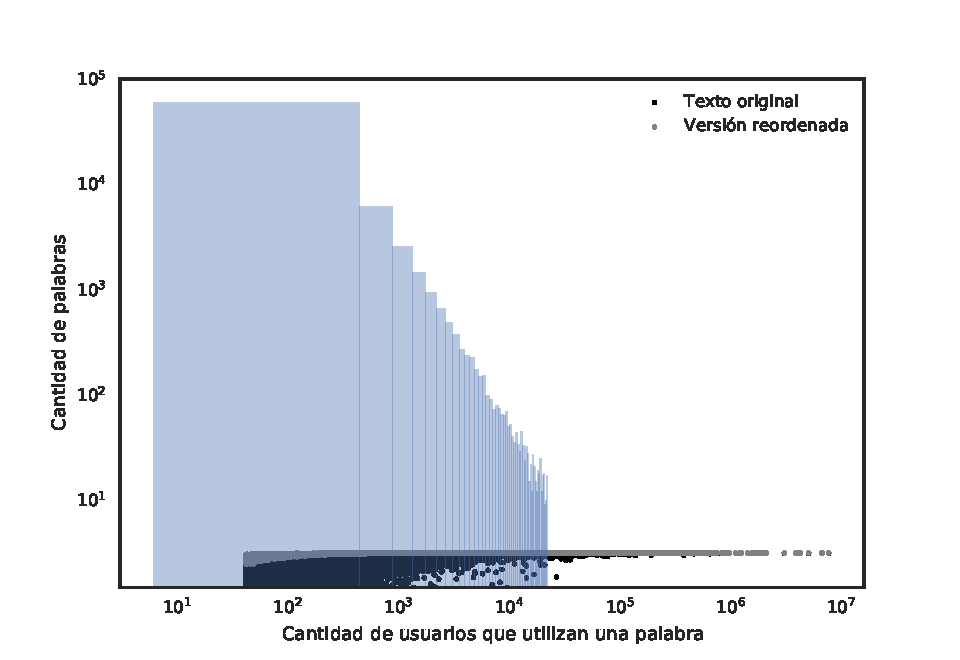
\includegraphics[width=\linewidth]{images2/cantUsuarios.pdf} 
    \caption{}
    \label{fig:cantUsuarios} 
   \end{subfigure}
   \caption{\subref{fig:cantPalabrasAnotaciones} Histograma de la cantidad de ocurrencias de las palabras. \subref{fig:cantUsuarios} Histograma de la cantidad de usuarios que utilizan una determinada cantidad de palabras.} 
   \label{fig:cantPalabrasSinNorm} 
\end{figure}

Para eliminar los valores atípicos se procedió a remover tanto las palabras que no superaran las 40 ocurrencias, como también aquellas que eran dichas por menos de 6 usuarios. La métrica se evaluó en este conjunto filtrado de palabras. En la Tabla \ref{tab:palabras_ivalue} se muestran las 20 palabras más contrastivas de acuerdo a nuestra métrica.

\subsection{Frecuencia de las palabras}
\label{sub: frecuenciaPalabras}
% Ver si se hace este gráfico con todas las palabras ya que por ahora tengo el conjunto de palabras con más de 40 ocurrencias
En la Figura \ref{fig:cantPalabrasAnotaciones} graficamos la distribución de la cantidad de ocurrencias de las palabras. Podemos observar que la mayoría de las palabras ocurren poco. En particular el 50\% de las palabras tienen una frecuencia relativa menor a $7.22e-07$. Por otro lado hay pocas palabras que ocurren mucho, por ejemplo la palabra \textit{que} o la preposición \textit{de}. En la Tabla \ref{tab:palabrasMasOcurrentes} del apéndice se encuentran las 20 palabras más frecuentes.


\begin{figure}[!ht]\centering
  \begin{subfigure}[t]{0.49\textwidth}
    \includegraphics[width=\linewidth]{./images2/cantNormUsuarios_sinFiltro.pdf}
    \caption{} 
    \label{fig:cantNormUsuarios} 
   \end{subfigure}
   \begin{subfigure}[t]{0.49\textwidth}
    \includegraphics[width=\linewidth]{images2/cantNormPalabras_sinFiltro.pdf}
    \caption{} 
    \label{fig:cantNormPalabras} 
   \end{subfigure}
   \caption{\subref{fig:cantNormUsuarios} Histograma de la normalización sobre la cantidad de usuarios que utilizan una determinada cantidad de palabras definida como $norm_p$. \subref{fig:cantNormPalabras} Histograma de la normalización de la cantidad de ocurrencias de las palabras definida como $norm_w$.}
   \label{fig:cantNormFig}
\end{figure}



\begin{table}[ht]
\centering
\begin{tabular}{@{}cc@{}}
\toprule
Palabra   & $I(w)$     \\ \midrule
chivilcoy & 1.533974 \\
oberá     & 1.491781 \\
ushuaia   & 1.461703 \\
ush       & 1.434766 \\
obera     & 1.244550 \\
breñas    & 1.227546 \\
viedma    & 1.213424 \\
bragado   & 1.202022 \\
logroño   & 1.188416 \\
nqn       & 1.143036 \\
tdf       & 1.126729 \\
riojanos  & 1.121459 \\
charata   & 1.071503 \\
chivil    & 1.043653 \\
cldo      & 1.036830 \\
blv       & 1.005322 \\
rioja     & 1.002387 \\
choele    & 0.999114 \\
tolhuin   & 0.985641 \\
rada      & 0.965216 \\ \bottomrule
\end{tabular}
\caption{Las 20 palabras más contrastivas de acuerdo a nuestra métrica $I(w)$.}
\label{tab:palabras_ivalue}
\end{table}

Si comparamos la posición de la palabra en un listado ordenado podemos ver que  las cantidades de ocurrencias parecieran seguir una distribución zipfiana. La ley de Zipf es una ley empírica formulada por George Zipf en el año 1932 en la cual se establece una relación entre la frecuencia de una palabra con su posición dentro del listado de palabras ordenadas por frecuencia decreciente \cite{montemurro2001beyond, zipf2016human}. En particular, sea $n$ la posición de la palabra en el listado ordenado y sea $f(n)$ la cantidad de ocurrencias de la n-ésima palabra, se puede hacer la siguiente aproximación:

$$f(n) \approx \frac{A}{n^{\alpha}}$$
donde $\alpha$ toma un valor levemente mayor a 1 y $A$ es una constante normalizadora.
Entonces, bajo la ley de Zipf uno puede saber que la frecuencia de la segunda palabra más dicha en un corpus es aproximadamente la mitad que la primera. La palabra con posición 3 en el listado ordenado por frecuencias, va a tener aproximadamente la tercera parte de la cantidad de ocurrencias que la primera y así sucesivamente. De esta manera hay una relación lineal entre el logaritmo de la posición del listado ordenado por frecuencias y el logaritmo de la cantidad de ocurrencias de cada palabra. Realizando una regresión lineal pesada según las cantidades de ocurrencias de las palabras obtuvimos un valor de $\alpha = 1,089$.

% TODO: escribirlo en ecuación,
Otra forma de utilizar esta ley empírica es la siguiente:
sabiendo la posición de una palabra $w$ en el listado ordenado por frecuencias de un corpus \textbf{A} y sabiendo la cantidad de palabras totales de un corpus \textbf{B}, puede estimarse la cantidad de ocurrencias de $w$ en el corpus \textbf{B}.
%TODO: HACER EJEMPLO de calculo de frecuencias a traves de la frecuencia de nuestro corpus


\begin{figure}[!ht]
\centering
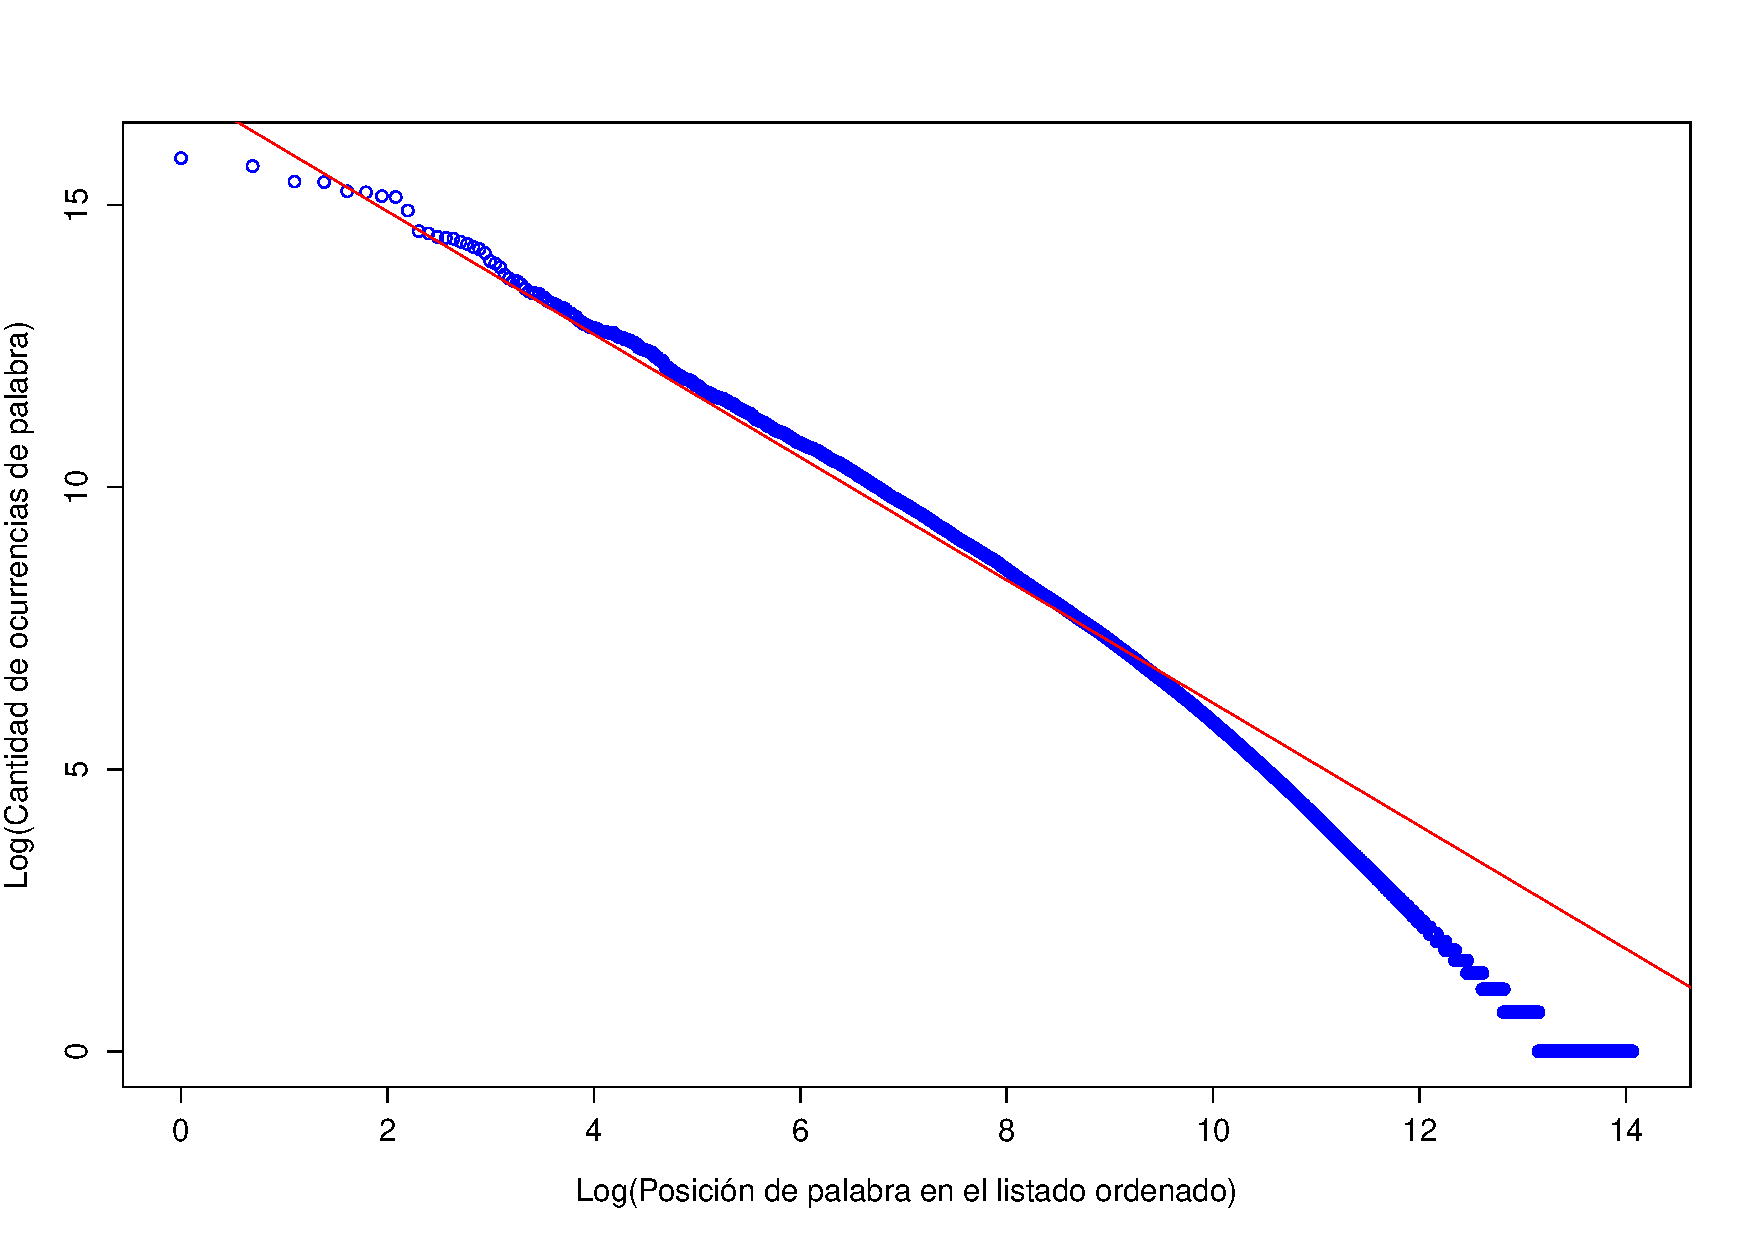
\includegraphics[width=0.5\textwidth]{images/zipfTodas.pdf}
\caption{Cantidad de ocurrencias de palabra vs posición en listado ordenado. Se aplicó el logaritmo natural a las cantidades de ocurrencias, como también a los valores de las posiciones para mostrar la proporcionalidad entre $f(n)$ y $\frac{1}{n^{\alpha}}$, obteniendo un valor de $\alpha=1.089$. } 
\label{fig:zipf} 
\end{figure}



%Qué resultados obtuvimos del análisis en cuestión. Acá vamos a poner qué palabras fueron significativas, dónde lo fueron, y demás.

% Distribucion de entropía vs frecuencia  
% Distribucion de frecuencias de las palabras
% Distr entropia
% de valor de la inf. a partir de los 5000 se ve que se estanca (graficar hasta 10**5)

% subsection de la region de las palabras --> muestro tabla
% se muestra que las regiones son contiguas geograficamente (hablarlo con santiago)

% Las palabras que se vieron, las primeras generalmente se refieren a lugares o gentilicios



% ver los graficos que hace zanette en su paper

% se busco el dataset de localidades para filtrar las palabras que son lugares

\section{Distribución de la entropía}
Teniendo el listado de palabras, hicimos un cálculo de entropía tomando en cada provincia la cantidad de ocurrencias de cada palabra. En la Figura \ref{fig:entropiaPalabras} podemos observar la distribución del valor de la entropía sobre todas las cantidades de ocurrencias de las palabras con más de 40 apariciones y dichas por más de 5 usuarios. 

Podemos ver que la mayor parte de las palabras tienen un valor de entropía entre 2.5 y 3. Esto quiere decir que hay un gran conjunto de palabras que tiene una cantidad de ocurrencias relativamente uniforme a lo largo de todas las provincias. 

Sin embargo, hay otro conjunto de palabras que tienen una entropía menor a 2, la cual podemos considerar como baja. Estas últimas palabras serán las que tienen mayor interés debido a que tienen una variación marcada en cuanto a su utilización en las distintas regiones. El máximo valor alcanzado de la entropía es de $3.1350$ con la palabra \textit{el}. Como aclaración la entropía calculada se realizó con logaritmos naturales, por lo tanto el máximo valor posible es de  $ln(23) = 3.1355$ donde habría una distribución uniforme en la cantidad de ocurrencias sobre las 23 provincias argentinas.

Tener en cuenta únicamente a la entropía de las palabras nos puede generar la detección de palabras que no son de interés, ya sea porque no ocurren una cantidad significativa de veces o porque la variación de las ocurrencias en las distintas provincias se debe solamente a pocos usuarios que la utilizan mucho. Es por esto que también se calculó la entropía teniendo como variable la cantidad de personas que usaron cierto término en una determinada provincia.


\begin{figure}[ht]
\centering
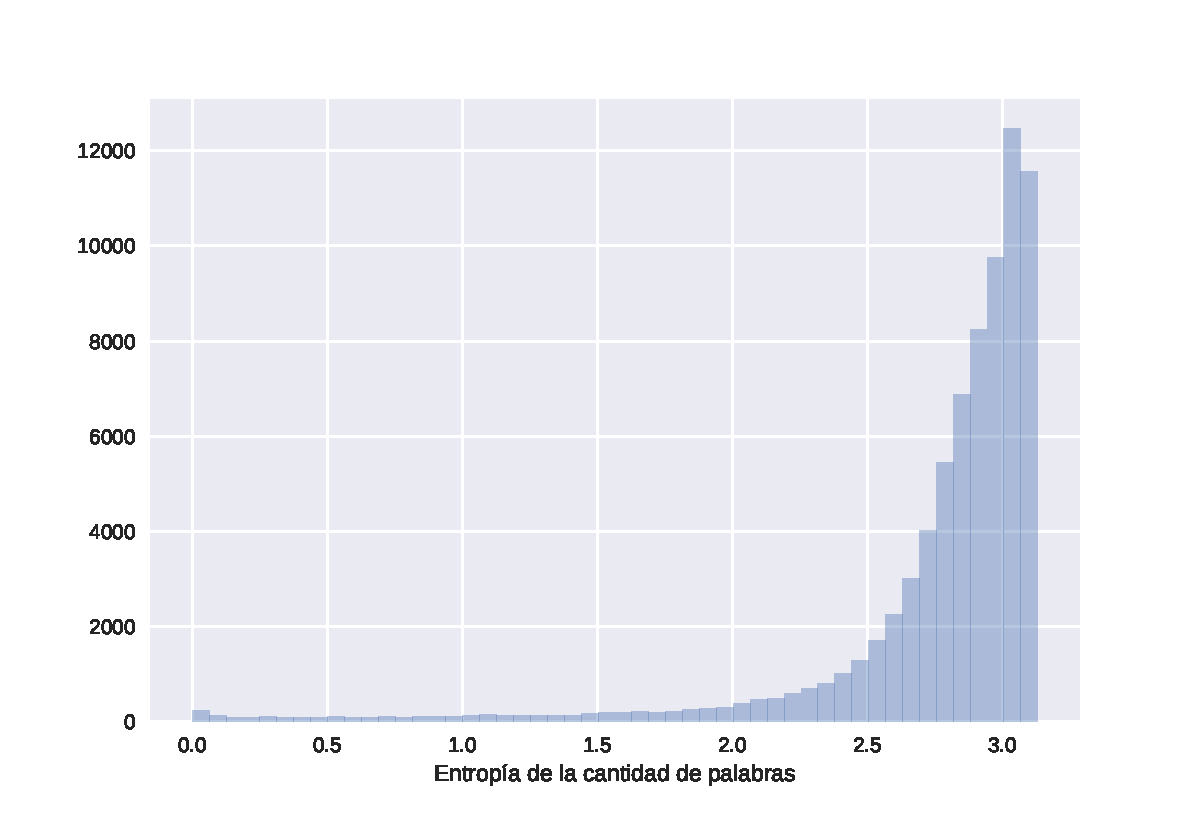
\includegraphics[width=0.9\textwidth]{./images/DistribucionEntropia.pdf}
\caption{Histograma del valor de la entropía de las palabras ($H_w$).} 
\label{fig:entropiaPalabras} 
\end{figure}

\section{Distribución del valor de contrastividad}
\label{sec:ValorDeLaInformacion}
En la Figura \ref{fig:infoValue} se muestra una clara relación entre la cantidad de ocurrencias que tiene una palabra y su valor de contrastividad definido en la ecuación \ref{eq:ivalor} , indicado por el color: cuanto más oscuro, más alto el valor. A su vez, se nota que el \textit{valor de contrastividad} suele ser mayor a medida que el valor de la entropía es menor. Esto no sucede siempre debido a que hay palabras que tienen una entropía de palabras $H_w$ baja, pero sin embargo la entropía de personas $H_p$ es alta, lo cual hace que el valor de contrastividad sea bajo.



\begin{figure}[!ht]\centering
  \begin{subfigure}[t]{0.49\linewidth}
    \centering
\includegraphics[width=0.95\textwidth]{./images2/entropiaPersonasxNormCantPersonasViridis.pdf}
\caption{} 
\label{fig:infoValue} 
  
   \end{subfigure}
   \begin{subfigure}[t]{0.49\linewidth}
      \centering
\includegraphics[width=0.95\textwidth]{./images2/valorInformacionCorte.pdf}
\caption{} 
\label{fig:ivalue}
  \end{subfigure}
   \caption{\subref{fig:infoValue} Gráfico de dispersión que muestra la posición en el listado ordenado según el valor de contrastividad reflejado por la escala cromática. A su vez se muestra para cada palabra el valor de la entropía de las personas ($H_p$) y la cantidad normalizada de personas que utiliza dicho término($norm_p$). \subref{fig:ivalue} Valor de contrastividad según la posición de la palabra en el listado de palabras. El gráfico se realizó sobre el conjunto de palabras cuya cantidad de ocurrencias era mayor a 40 y la cantidad de usuarios que utilizaron cada término era mayor a 5. Desde la palabra cuya posición es 4000, el valor $I$ se estabiliza alrdededor de 0.}
   \label{fig:infoeivalue}
\end{figure}

% \begin{figure}[h]
% \centering
% 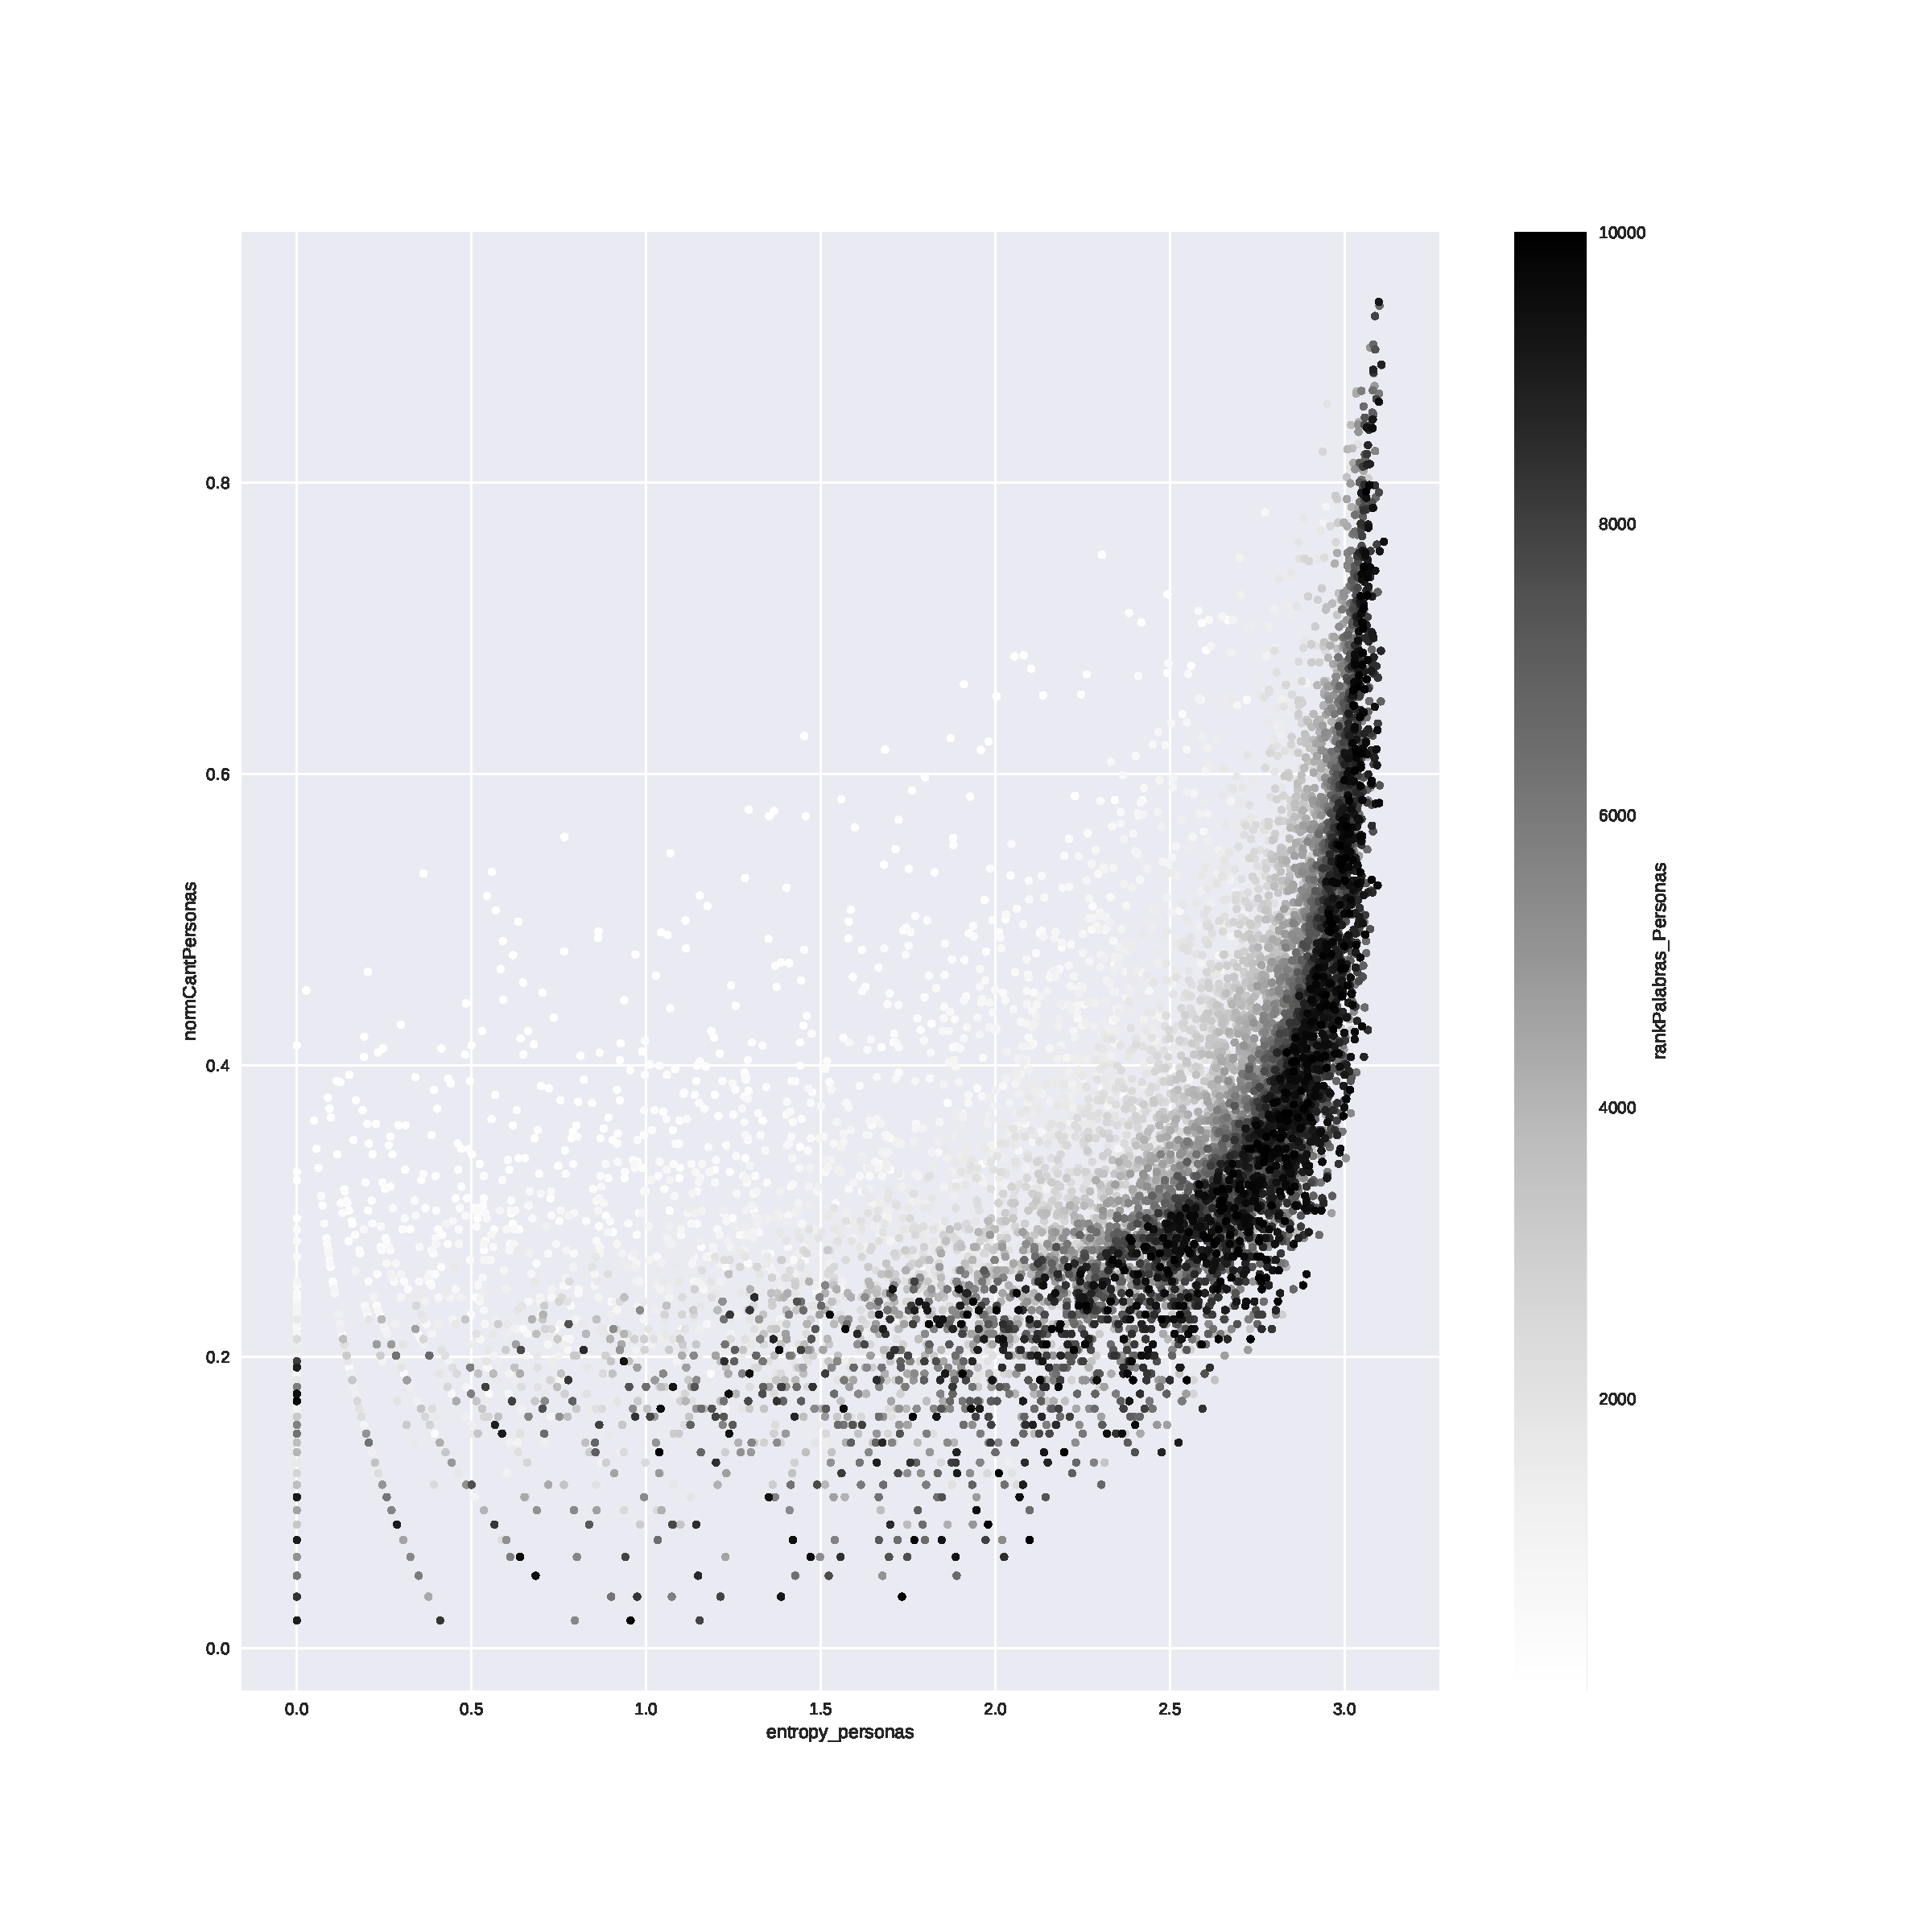
\includegraphics[width=0.9\textwidth]{./images2/entropiaPersonasxNormCantPersonas.pdf}
% \caption{Gráfico de dispersión que muestra la posición en el listado ordenado según el valor de contrastividad reflejado por la escala cromática. Las posiciones más bajas aparecen más blancas. A su vez se muestra para cada palabra el valor de la entropía de las personas ($H_p$) y la cantidad normalizada de personas que utiliza dicho término($norm_p$). } 
% \label{fig:infoValue} 
% \end{figure}

En la Figura \ref{fig:ivalue} se puede ver el valor de contrastividad según la posición en la que se encuentra en el listado ordenado por la métrica. Notamos que el valor se estabiliza aproximadamente a partir de la palabra en la posición número 4000, a partir de donde tiende a acercarse a 0.


% \begin{figure}
% \centering
% \includegraphics[width=0.9\textwidth]{./images/train/conFiltro/valorInformacionCorte.pdf}
% \caption{Distribución del valor de contrastividad según la posición de la palabra en el listado de palabras. El gráfico se realizó sobre el conjunto de palabras cuya cantidad de ocurrencias era mayor a 40 y la cantidad de usuarios que utilizaron cada término era mayor a 5. } 
% \label{fig:ivalue}
% \end{figure}



\section{Proporción acumulada de ocurrencias} % (fold)
\label{sec:proporcionDeOcurrencias}
Además de la detección de las palabras contrastivas en su uso, nos interesa saber en qué regiones se utilizan más. Para esto ordenamos, por cada palabra, las provincias de acuerdo a la cantidad de menciones, formando una lista de provincias: $ps = p_1,p_2,\ldots,p_{23}$, 
donde $\#w(p_1) \geq \#w(p_2) \ldots \#w(p_{23})$. Luego elegimos al conjunto de provincias que superen un cierto porcentaje de todas las ocurrencias.
Esto lo realizamos en distintas muestras de palabras, las 1000-2000-5000-10000 más contrastivas según nuestra métrica y sobre el conjunto total de las palabras(sin incluír a las palabras que son dichas por menos de 5 usuarios o con menos de 40 ocurrencias en todo el conjunto de datos). Reflejamos este análisis en la Figura \ref{fig:propAcum} donde cada curva representa la proporción acumulada media según la cantidad de provincias, eligiendo por cada palabra y una cantidad de provincias determinada aquel conjunto de provincias que maximice la proporción. Es notable la diferencia de proporciones acumuladas según la muestra de palabras. Solamente con una provincia para cada palabra ya se puede cubrir, en promedio, el 76\% del total de ocurrencias sobre las mil palabras con mayor valor de nuestra métrica.

En el gráfico de la Figura \ref{fig:propAcum5000} se observa que la variación del cubrimiento de ocurrencias disminuye a medida que se aumenta la cantidad de provincias tomando la muestra con las primeras 5000 palabras con mayor valor de contrastividad. 

% Para identificar cuál debiera ser ese porcentaje hicimos lo siguiente: por cada palabra, calculamos el porcentaje de ocurrencias sobre los conjuntos de $n$ provincias, variando $n$ de $1$ a $23$, a partir de la lista $ps$ de provincias ordenadas. Es decir, por cada región formada por una determinada cantidad de provincias calculamos el mayor porcentaje posible de ocurrencias de una palabra dada.
% En la Figura \ref{fig:propAcum} mostramos la proporción acumulada de las palabras, tomando diferentes muestras de palabras. Es notable la diferencia de proporciones acumuladas según la muestra de palabras. Solamente con una provincia para cada palabra ya se puede cubrir, en promedio, el 76\% del total de ocurrencias sobre las mil palabras con mayor valor de nuestra métrica.

% En el gráfico de la Figura \ref{fig:propAcum5000} se observa que la variación del cubrimiento de ocurrencias disminuye a medida que se aumenta la cantidad de provincias. 




% \begin{figure}[!ht]\centering
%   \begin{subfigure}[t]{0.49\textwidth}
%     \includegraphics[width=0.95\textwidth]{images/PropAcumSinCandidatas.pdf}
%     \caption{} 
%     \label{fig:propAcum}  
%    \end{subfigure}
%    \begin{subfigure}[t]{0.49\textwidth}
%        \includegraphics[width=0.95\textwidth]{images/PropAcum5000SinCandidatas.pdf}
%     \caption{} 
%     \label{fig:propAcum5000} 
%   \end{subfigure}
%    \caption{\subref{fig:propAcum} Proporción de ocurrencias acumulada según la muestra de palabras. El número de la leyenda indica la cantidad de palabras contrastivas elegidas para la muestra respectiva, siempre seleccionando las más contrastivas según la métrica. \subref{fig:propAcum5000} Variación de la proporción de ocurrencias acumulada a partir de la muestra con las primeras 5000 palabras con mayor valor de contrastividad.}
%    \label{fig:propAcums}
% \end{figure}


\begin{figure}[ht]\centering
    \includegraphics[width=0.62\textwidth]{images/PropAcumSinCandidatas.pdf}
    \caption{Proporción de ocurrencias acumulada media según la muestra de palabras. El número de la leyenda indica la cantidad de palabras contrastivas elegidas para la muestra respectiva, siempre seleccionando las más contrastivas según la métrica. En cada curva se refleja el promedio de la proporción acumulada de una muestra variando la cantidad de provincias que forman las regiones maximales.} 
    \label{fig:propAcum} 
\end{figure}


\begin{figure}[h]\centering
    \includegraphics[width=0.62\textwidth]{images/PropAcum5000SinCandidatas.pdf}
    \caption{Variación de la proporción de ocurrencias acumulada a partir de la muestra con las primeras 5000 palabras con mayor valor de contrastividad.} 
    \label{fig:propAcum5000} 
\end{figure}

